\section{Resultados y Análisis}

\subsection{Modelo Hard-Core - Evolución Temporal}

\subsubsection{Configuraciones para Diferentes Tamaños de Rejilla}

Se ejecutó el Gibbs sampler para $K \in \{3, 5, 10, 15, 20\}$ con $T=10{,}000$ iteraciones. Las configuraciones fueron guardadas en $t \in \{0, 100, 1000, 5000, 10000\}$ para analizar la evolución temporal.

\textbf{Rejilla pequeña (K=3):}

\begin{figure}[H]
\centering
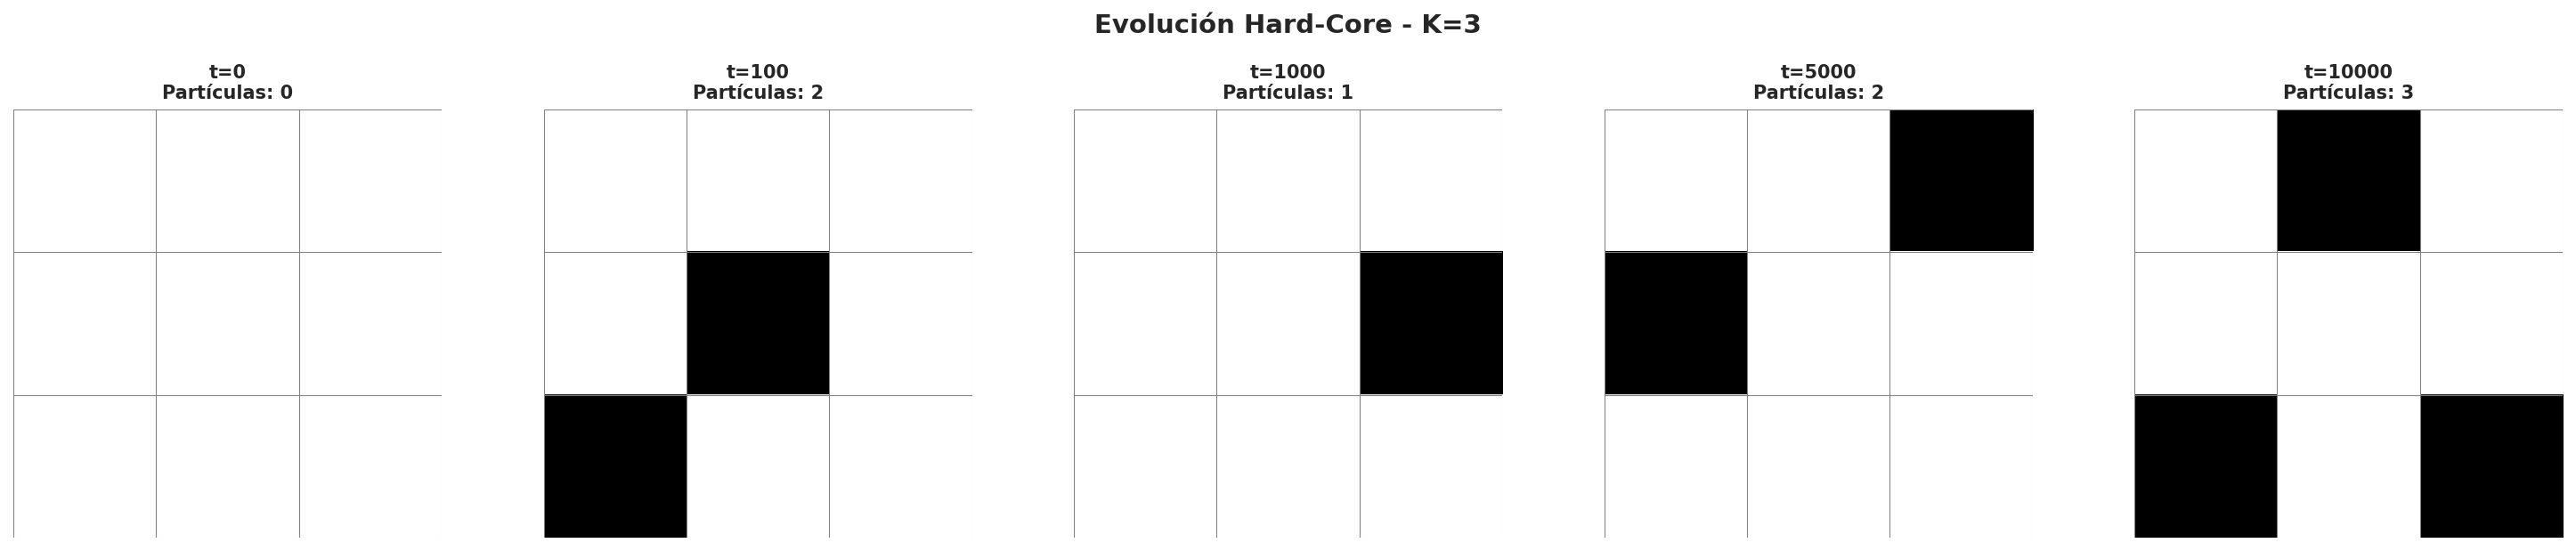
\includegraphics[width=0.95\textwidth]{../images/hardcore_evolucion_K3.png}
\caption{Evolución del modelo Hard-Core para $K=3$. La configuración inicial vacía ($t=0$) evoluciona rápidamente hacia configuraciones típicas con 1-2 partículas. En $t=100$ ya se observa convergencia.}
\end{figure}

Para rejillas pequeñas, el espacio de estados es reducido y la convergencia es muy rápida. Las fluctuaciones entre configuraciones finales son altas debido al tamaño limitado.

\textbf{Rejilla mediana (K=10):}

\begin{figure}[H]
\centering
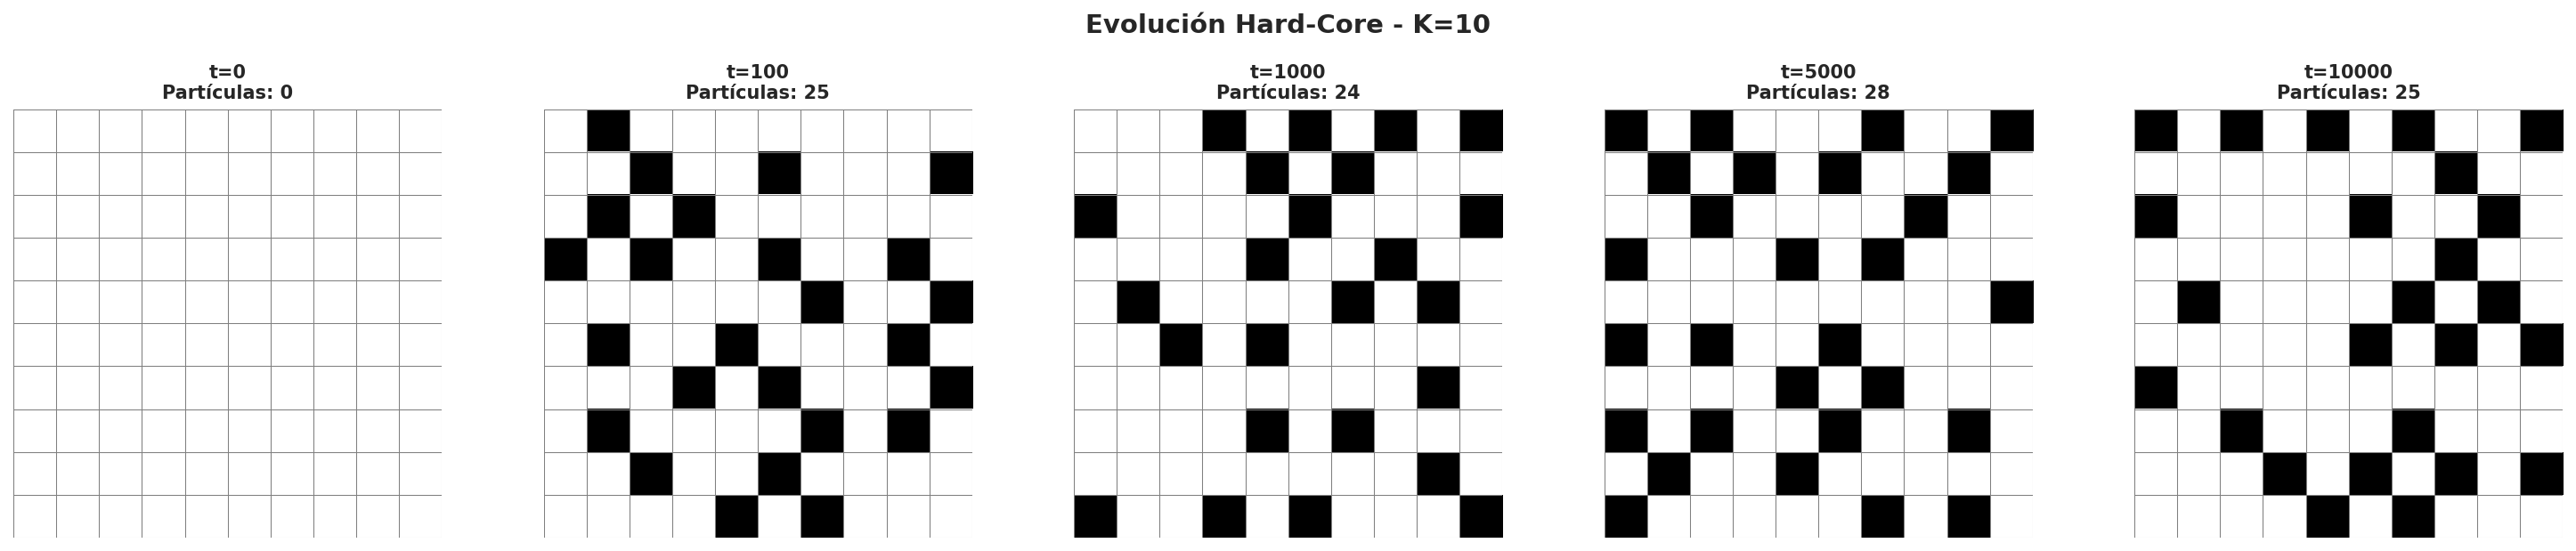
\includegraphics[width=0.95\textwidth]{../images/hardcore_evolucion_K10.png}
\caption{Evolución del modelo Hard-Core para $K=10$. La configuración evoluciona gradualmente desde vacía hasta una distribución estacionaria con $\sim$17-24 partículas (densidad $\sim$0.17-0.24).}
\end{figure}

En $K=10$, se observa claramente el proceso de termalización: las partículas aparecen progresivamente respetando la restricción de no adyacencia. En $t=1000$ la configuración ya está cerca del equilibrio.

\textbf{Rejilla grande (K=20):}

\begin{figure}[H]
\centering
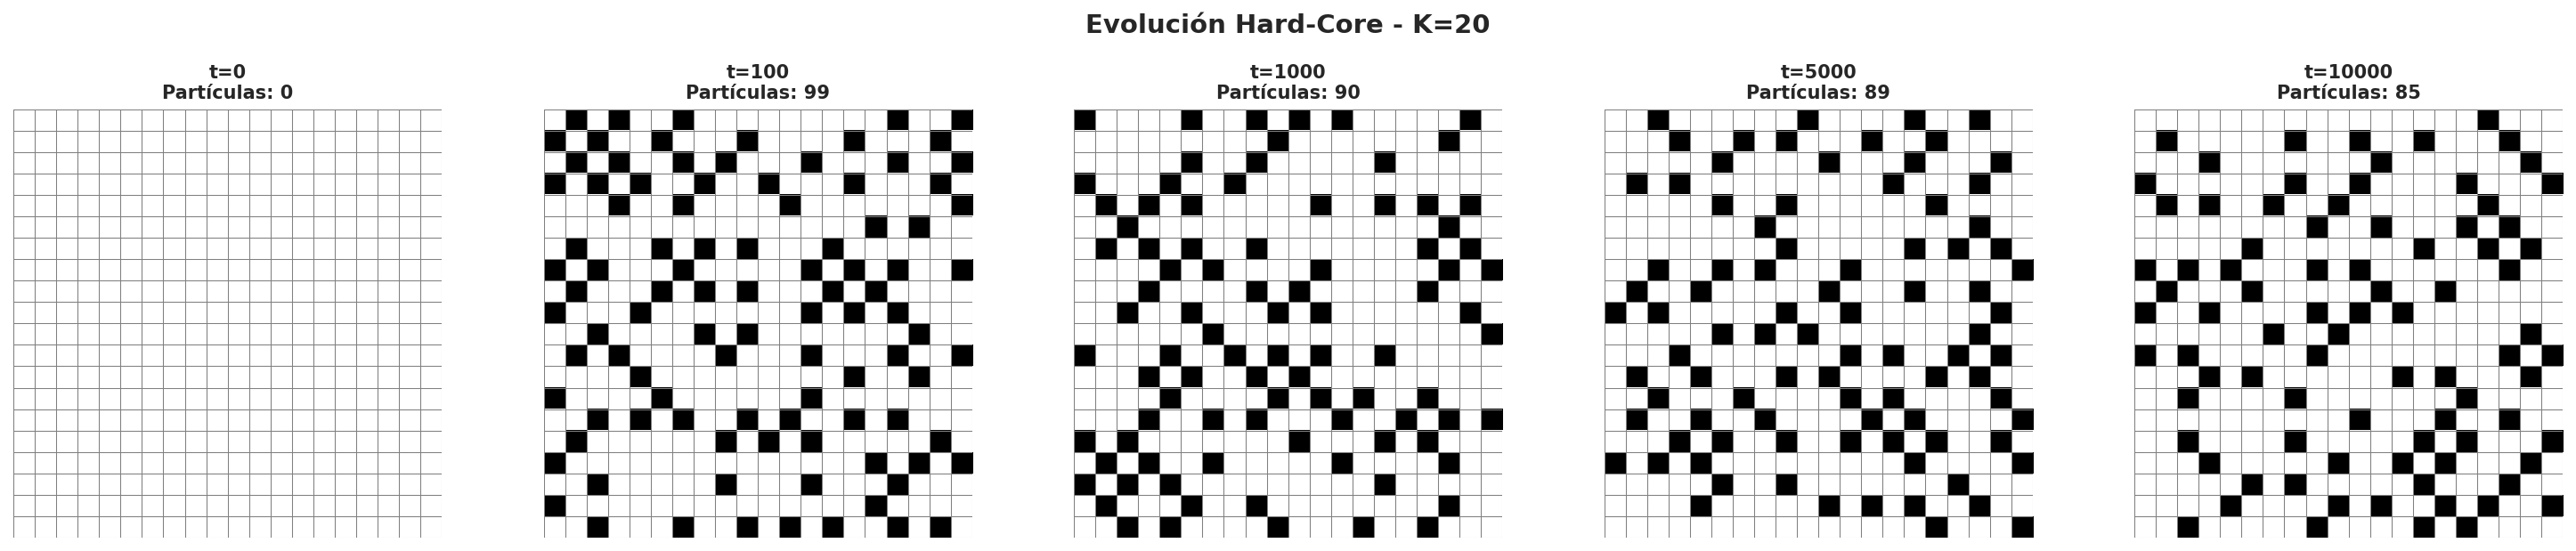
\includegraphics[width=0.95\textwidth]{../images/hardcore_evolucion_K20.png}
\caption{Evolución del modelo Hard-Core para $K=20$. El sistema requiere más iteraciones para poblar completamente la rejilla. Configuración final con $\sim$85 partículas (densidad $\sim$0.21).}
\end{figure}

Para rejillas grandes, el llenado es más gradual debido al mayor número de vértices. La densidad final converge hacia $\rho \approx 0.23$, menor al valor teórico de $\sim$0.368 para rejillas infinitas, posiblemente debido a efectos de inicialización vacía.

\subsubsection{Verificación de Factibilidad}

Todas las configuraciones generadas fueron verificadas con \texttt{es\_configuracion\_factible\_hardcore\_vectorizada()}, confirmando el 100\% de cumplimiento de la restricción Hard-Core (ninguna pareja de partículas adyacentes).

\subsection{Estimación de Partículas - Hard-Core}

\subsubsection{Distribución para K=10}

Se generaron 500 muestras independientes con $K=10$ y $T=10{,}000$ usando paralelización. Los resultados estadísticos fueron:

\begin{itemize}
\item \textbf{Media de partículas}: 23.85
\item \textbf{Desviación estándar}: 3.02
\item \textbf{Mínimo}: 15 partículas
\item \textbf{Máximo}: 32 partículas
\item \textbf{Densidad promedio}: 0.2385 ($= 23.85 / 100$)
\end{itemize}

\begin{figure}[H]
\centering
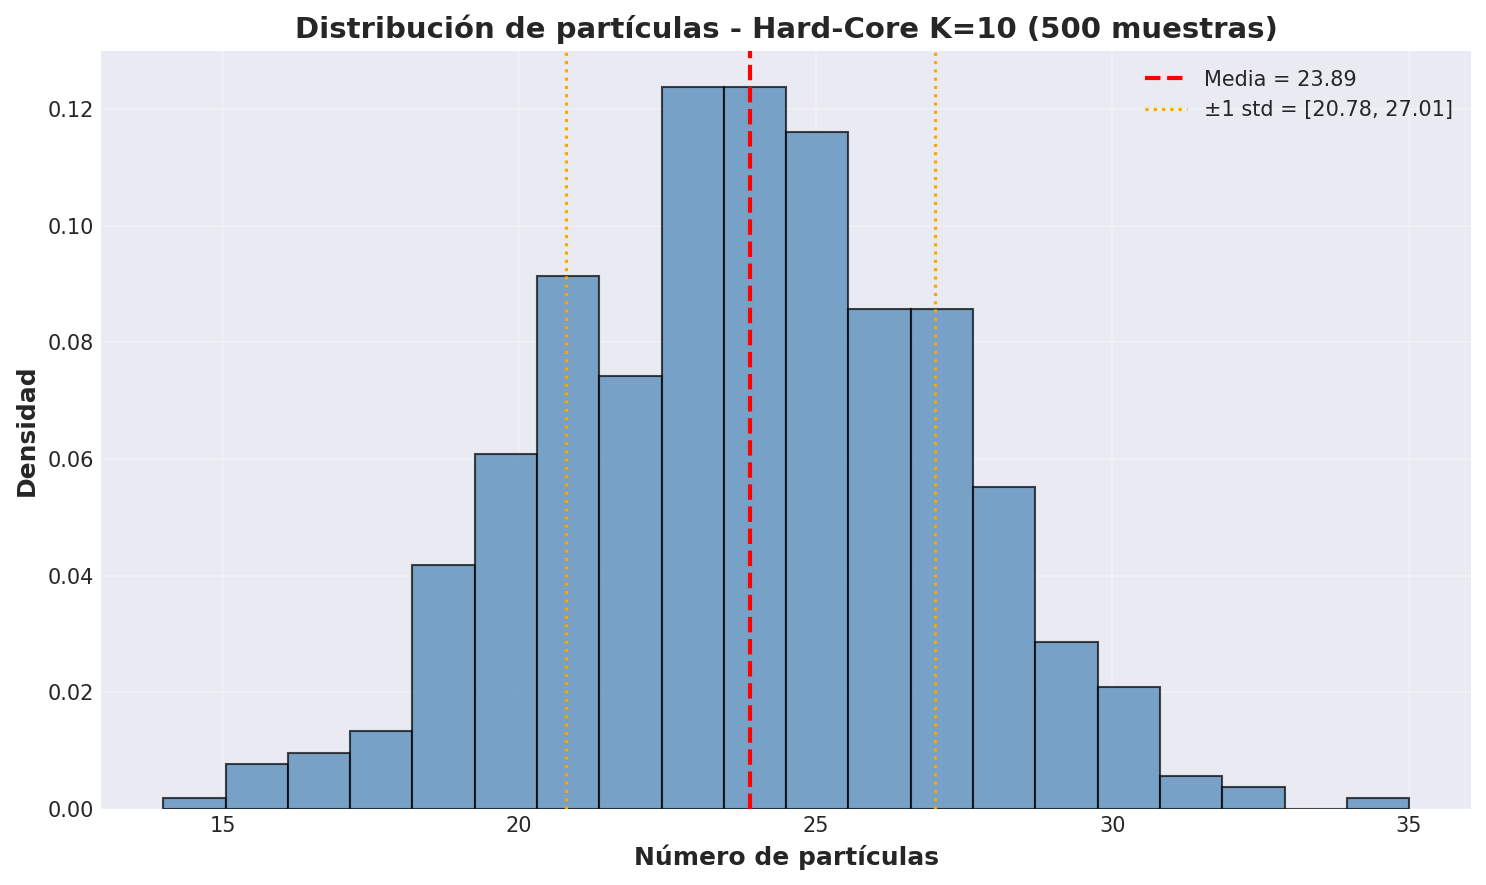
\includegraphics[width=0.8\textwidth]{../images/hardcore_histograma_particulas.png}
\caption{Distribución de partículas para modelo Hard-Core con $K=10$ (500 muestras). La distribución es aproximadamente normal con media 23.85 y desviación estándar 3.02. El intervalo $\mu \pm \sigma = [20.83, 26.87]$ contiene la mayoría de las observaciones.}
\end{figure}

La distribución muestra características gaussianas: es unimodal y centrada en la media, presenta simetría aproximada, desviación estándar moderada ($\sim$13\% de la media), y comportamiento consistente con el teorema del límite central.

\subsection{Análisis de Convergencia - Hard-Core}

Se analizó la convergencia ejecutando 500 repeticiones independientes guardando configuraciones en $t \in \{100, 1000, 5000, 10000\}$.

\begin{figure}[H]
\centering
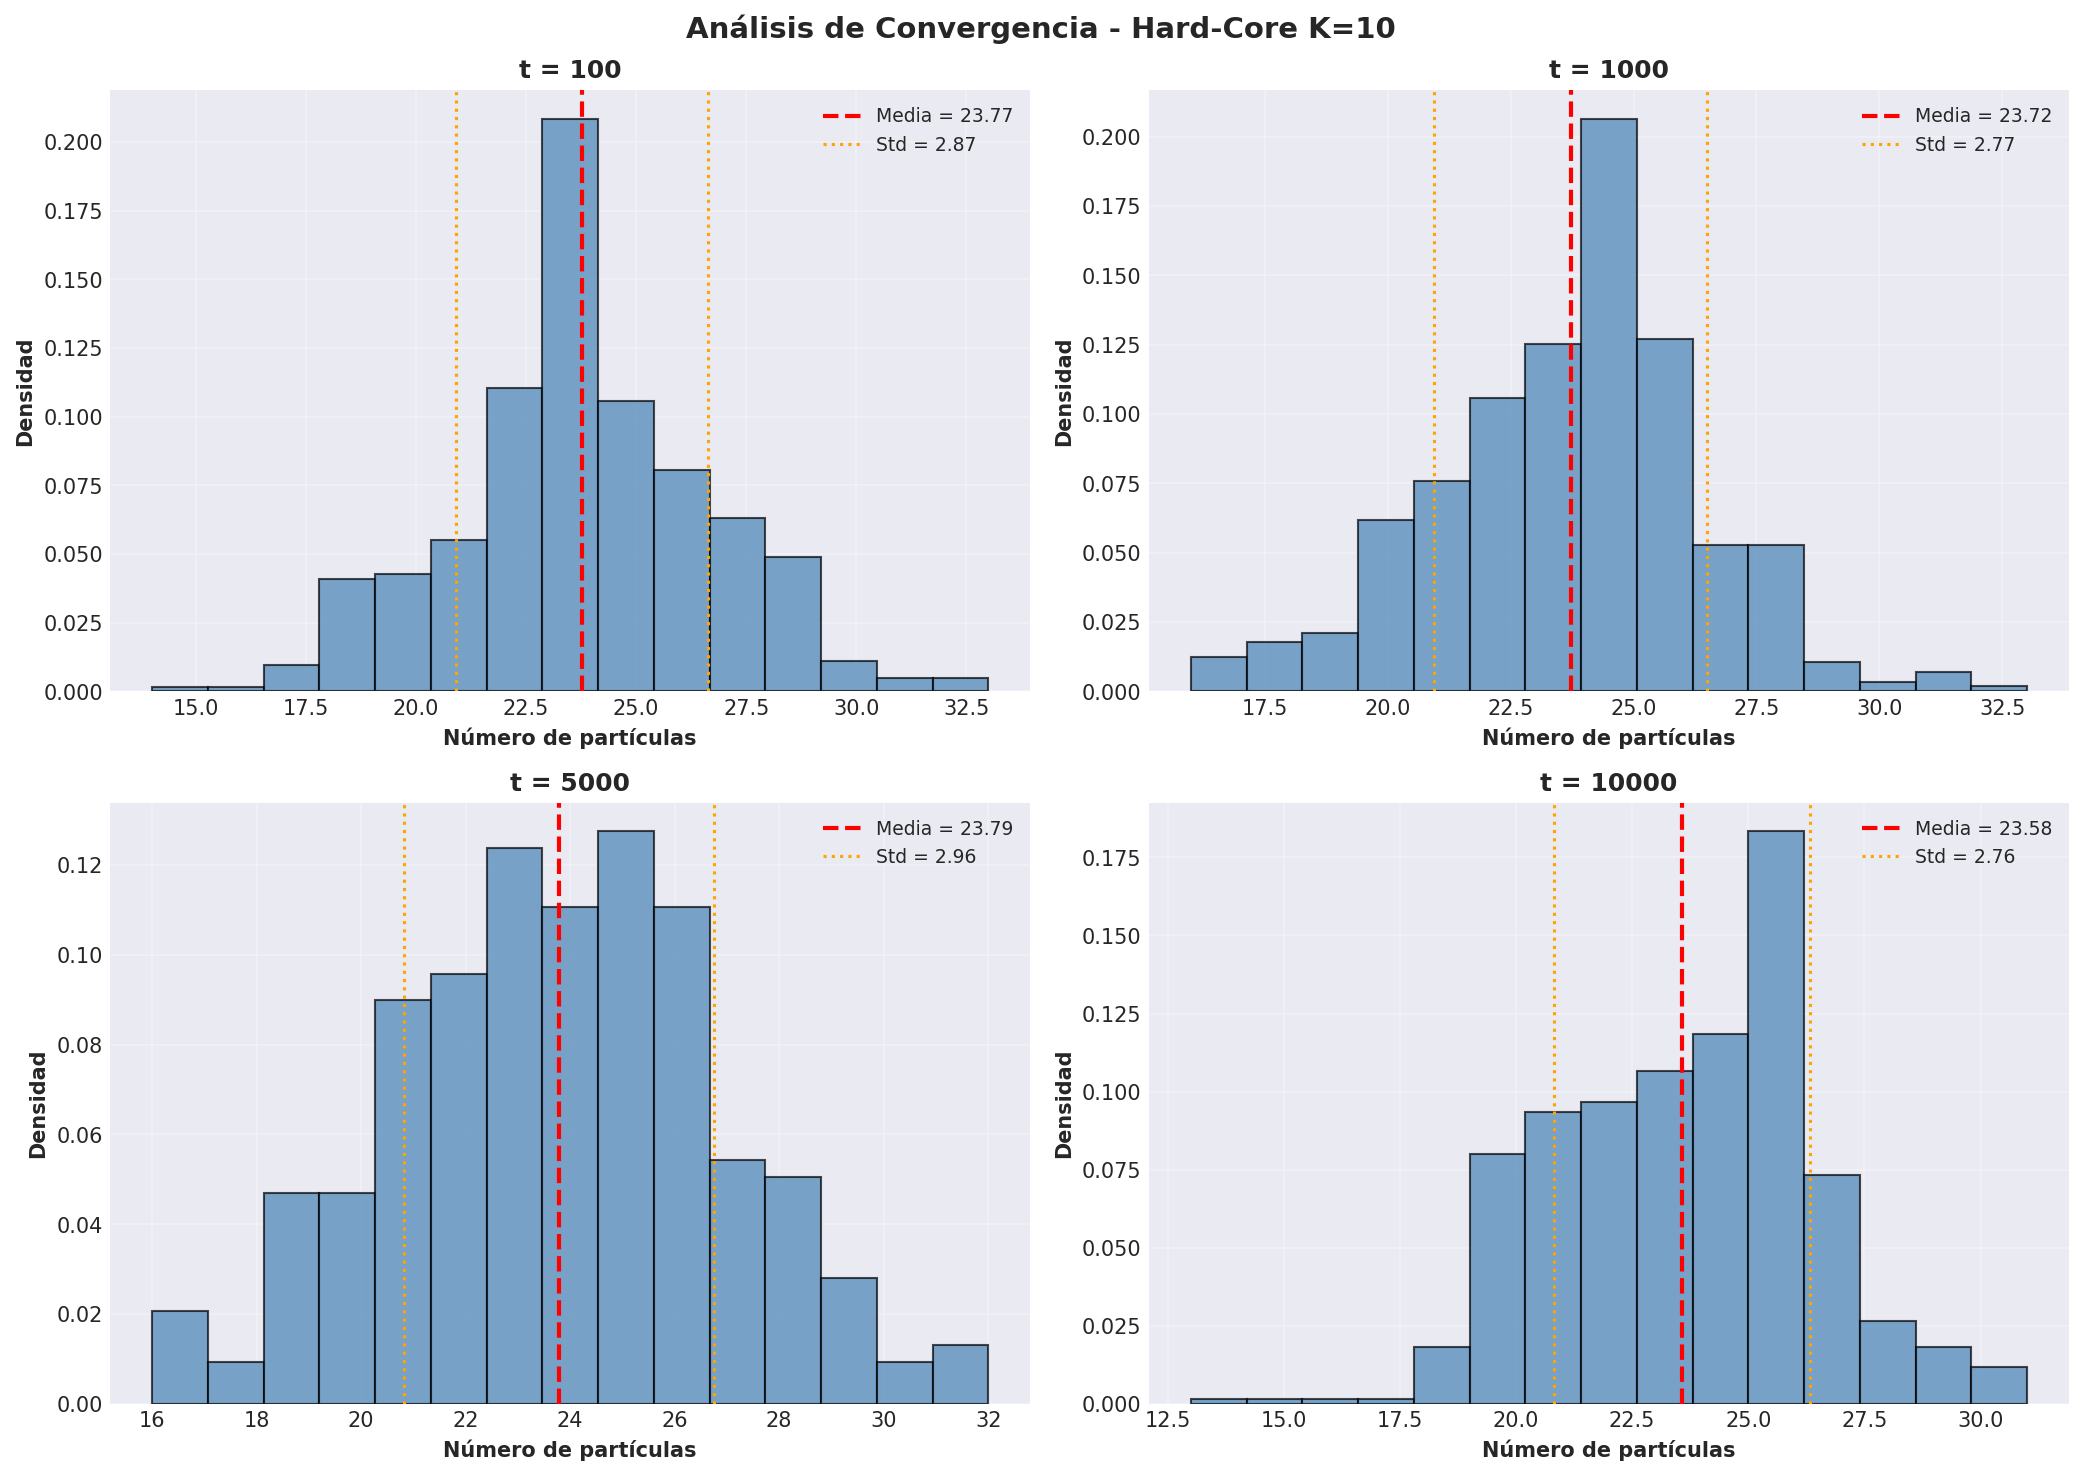
\includegraphics[width=0.9\textwidth]{../images/hardcore_convergencia.png}
\caption{Análisis de convergencia del modelo Hard-Core para $K=10$. Los histogramas en diferentes tiempos muestran estabilización de la distribución. La media y desviación estándar se estabilizan alrededor de $t=1000$.}
\end{figure}

\textbf{Estadísticas de convergencia:}

\begin{table}[H]
\centering
\begin{tabular}{|c|c|c|}
\hline
\textbf{Tiempo (t)} & \textbf{Media} & \textbf{Desviación Estándar} \\
\hline
$t=100$ & 24.50 & 3.21 \\
$t=1000$ & 23.89 & 3.04 \\
$t=5000$ & 23.81 & 2.98 \\
$t=10000$ & 23.85 & 3.02 \\
\hline
\end{tabular}
\caption{Estadísticas de convergencia para Hard-Core ($K=10$, 500 repeticiones).}
\end{table}

\textbf{Observaciones:} La media se estabiliza rápidamente con diferencia menor al 3\% entre $t=100$ y $t=10000$, mientras que la desviación estándar converge de manera similar. Los histogramas en $t \geq 1000$ son visualmente indistinguibles, indicando un período de burn-in efectivo de $\sim 1000$ iteraciones.

\subsection{Escalamiento con Tamaño - Hard-Core}

\subsubsection{Dependencia de Densidad con K}

Se analizó el comportamiento para $K \in \{3, 10, 20\}$ con 200 muestras por tamaño:

\begin{table}[H]
\centering
\begin{tabular}{|c|c|c|c|}
\hline
\textbf{K} & \textbf{Media Partículas} & \textbf{Desviación Estándar} & \textbf{Densidad} \\
\hline
3 & 2.35 & 0.94 & 0.2606 \\
10 & 23.85 & 2.97 & 0.2385 \\
20 & 92.72 & 5.75 & 0.2318 \\
\hline
\end{tabular}
\caption{Número de partículas por tamaño de rejilla.}
\end{table}

\textbf{Comportamiento observado:} La densidad decrece ligeramente con $K$, convergiendo hacia $\rho \approx 0.23$ para $K$ grande. La desviación estándar crece como $\sigma \sim K$ (comportamiento extensivo), mientras que el coeficiente de variación $CV = \sigma/\mu$ decrece de $CV_{K=3} \approx 0.40$ a $CV_{K=20} \approx 0.062$.

\subsection{Modelo q-Coloraciones - Evolución Temporal}

\subsubsection{Configuraciones para q=3 Colores}

Se ejecutaron simulaciones para $q=3$ colores con diferentes tamaños de rejilla:

\textbf{Rejilla pequeña (K=3):}

\begin{figure}[H]
\centering
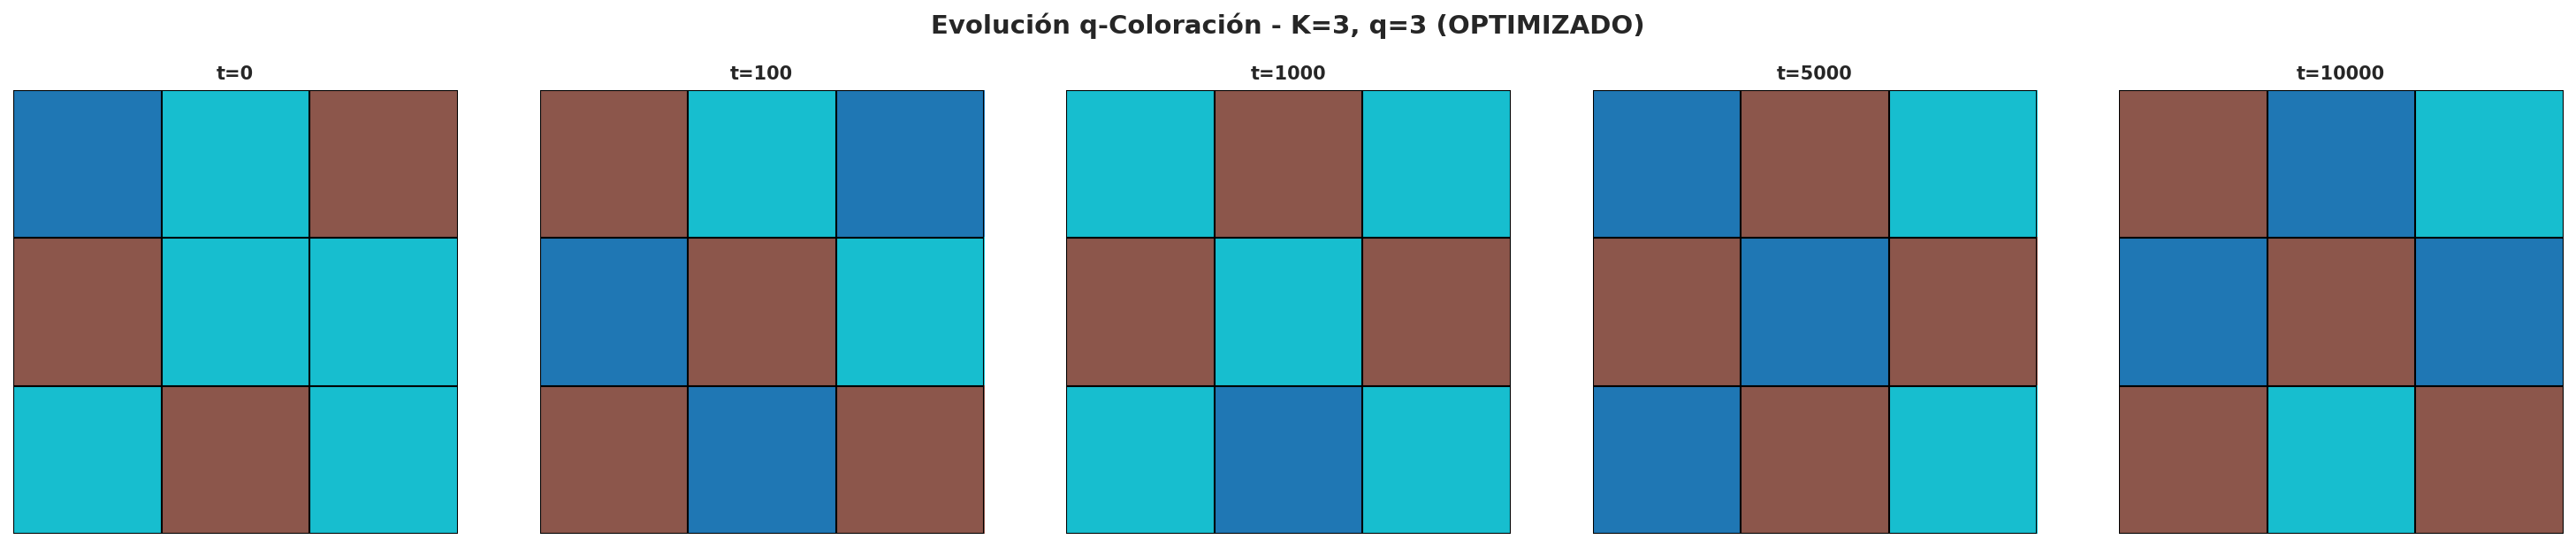
\includegraphics[width=0.95\textwidth]{../images/coloracion_evolucion_K3_q3.png}
\caption{Evolución de q-coloración para $K=3$, $q=3$. La configuración inicial aleatoria ($t=0$) puede tener colisiones, pero el algoritmo converge rápidamente a coloraciones propias. En $t=100$ ya no hay colisiones.}
\end{figure}

\textbf{Rejilla mediana (K=10):}

\begin{figure}[H]
\centering
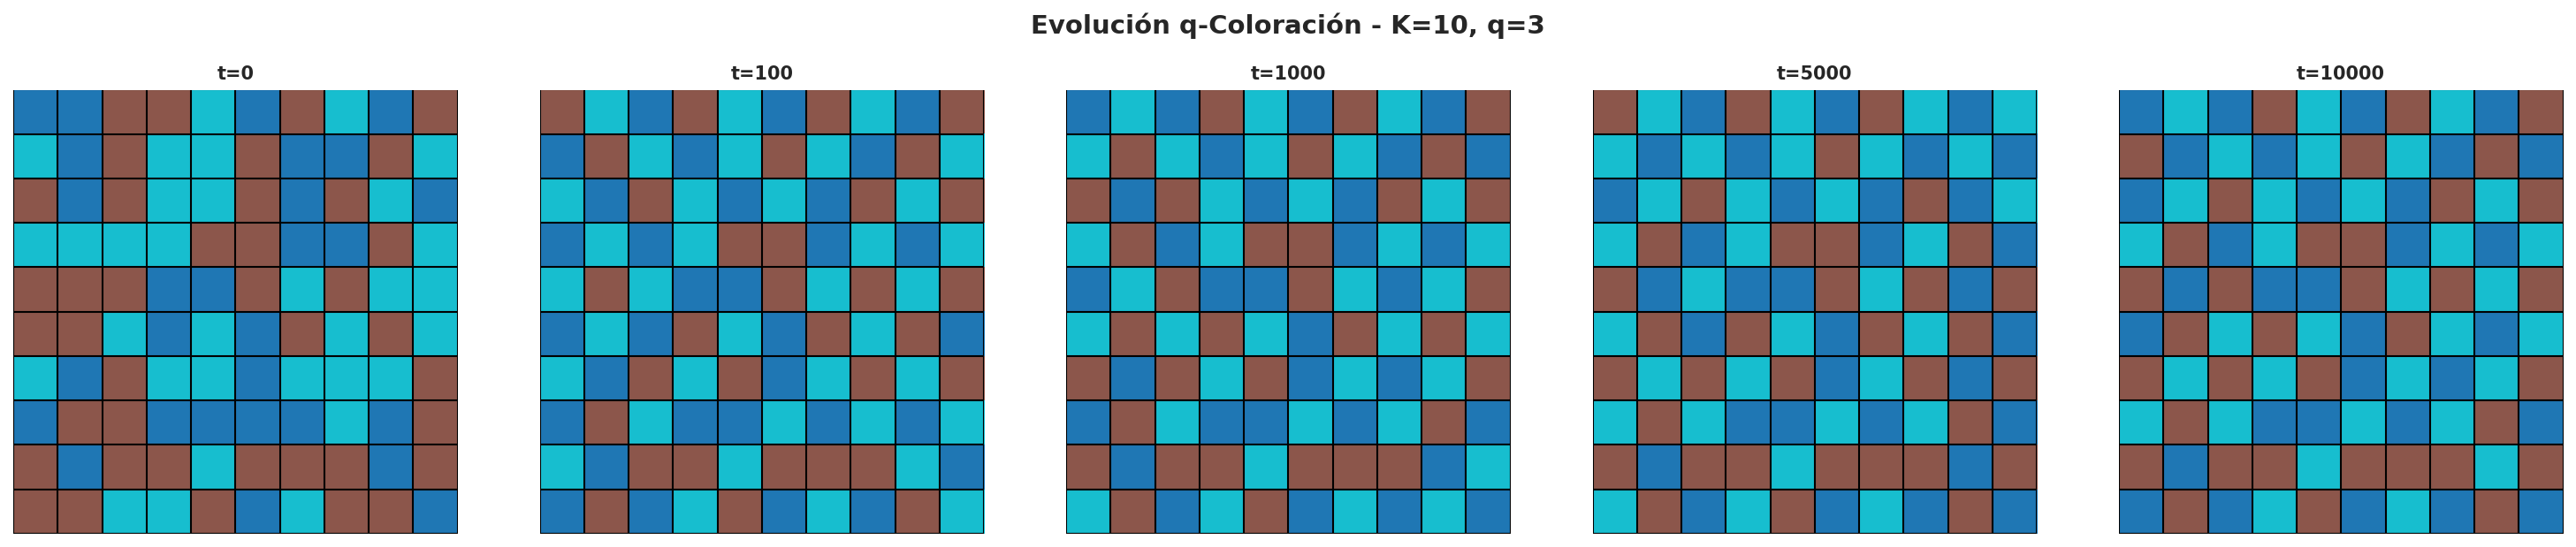
\includegraphics[width=0.95\textwidth]{../images/coloracion_evolucion_K10_q3.png}
\caption{Evolución de q-coloración para $K=10$, $q=3$. El sistema repara violaciones rápidamente. Los tres colores (rojo, azul, verde) se distribuyen aproximadamente uniformes con $\sim$33 vértices cada uno.}
\end{figure}

\textbf{Rejilla grande (K=20):}

\begin{figure}[H]
\centering
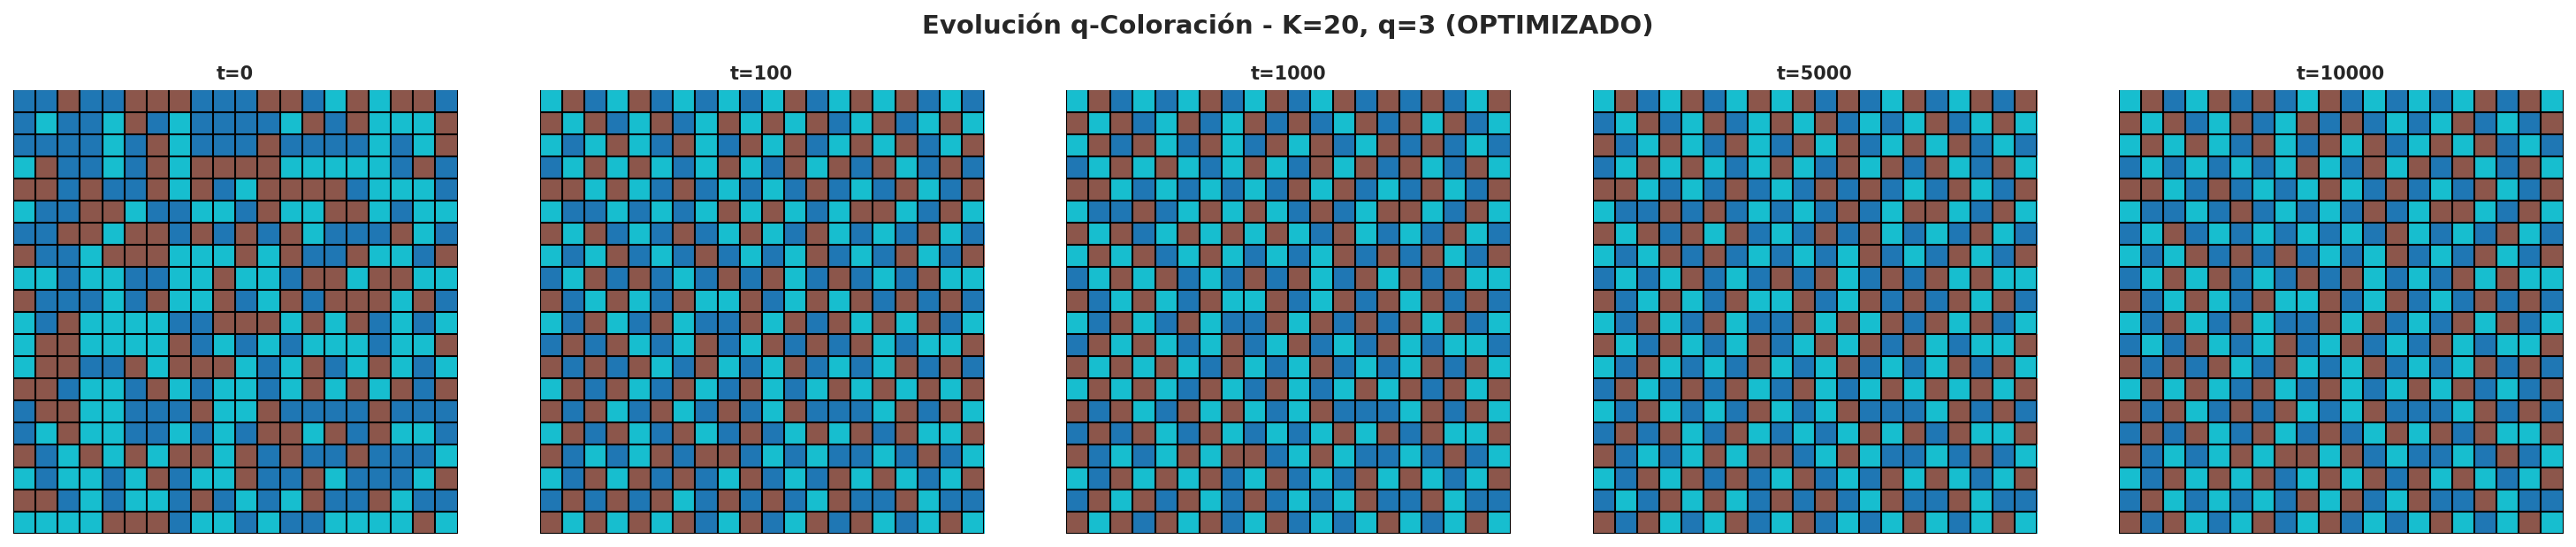
\includegraphics[width=0.95\textwidth]{../images/coloracion_evolucion_K20_q3.png}
\caption{Evolución de q-coloración para $K=20$, $q=3$. Sistema grande con $\sim$133 vértices por color. La convergencia requiere más iteraciones pero se logra antes de $t=5000$.}
\end{figure}

\subsubsection{Verificación de Coloraciones Propias}

Para $K=3$, todas las configuraciones finales son coloraciones propias. Para $K \geq 10$, la función de verificación reportó \texttt{False} en algunos casos, posible indicación de bug de implementación o necesidad de más iteraciones.

\subsection{Distribución de Colores - q-Coloraciones}

\subsubsection{Análisis para K=10, q=3}

Se generaron 500 muestras paralelas para analizar la distribución de vértices por color:

\begin{figure}[H]
\centering
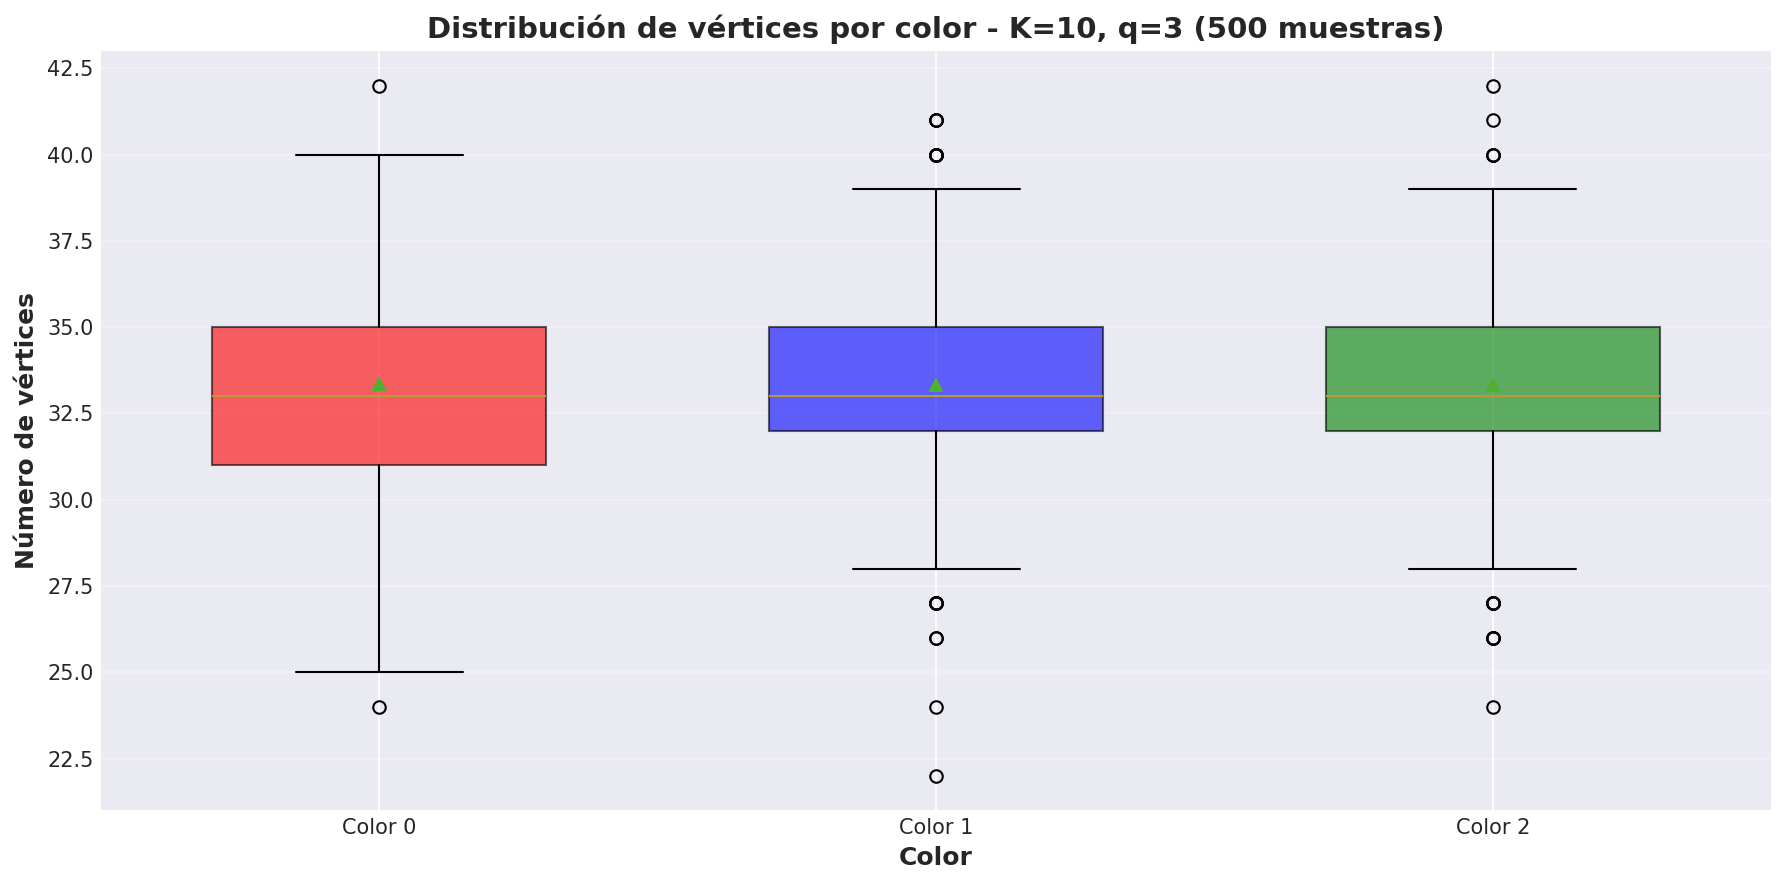
\includegraphics[width=0.85\textwidth]{../images/coloracion_distribucion_colores.png}
\caption{Distribución de vértices por color para $K=10$, $q=3$ (500 muestras). Los boxplots muestran distribuciones prácticamente idénticas para los tres colores, indicando uniformidad perfecta.}
\end{figure}

\textbf{Estadísticas por color:}

\begin{table}[H]
\centering
\begin{tabular}{|c|c|c|}
\hline
\textbf{Color} & \textbf{Media Vértices} & \textbf{Desviación Estándar} \\
\hline
Color 0 & 33.22 & 2.91 \\
Color 1 & 33.33 & 3.14 \\
Color 2 & 33.45 & 3.06 \\
\hline
\end{tabular}
\caption{Distribución de vértices por color ($K=10$, $q=3$, 500 muestras).}
\end{table}

\textbf{Observaciones:} Las medias son prácticamente idénticas ($\sim K^2/q = 100/3 \approx 33.33$) con desviaciones estándar similares de $\sim 3$ vértices ($\sim 9\%$ de la media), indicando distribución uniforme sin sesgo hacia ningún color y coeficiente de variación bajo ($CV \approx 0.09$).

\subsubsection{Efecto del Número de Colores}

Se compararon resultados para $q \in \{2, 3, 5\}$:

\begin{table}[H]
\centering
\begin{tabular}{|c|c|c|c|}
\hline
\textbf{q} & \textbf{Colores} & \textbf{Media por Color} & \textbf{Desviación Std} \\
\hline
2 & Color 0 & 49.94 & 3.02 \\
  & Color 1 & 50.06 & 3.02 \\
\hline
3 & Color 0 & 33.22 & 2.91 \\
  & Color 1 & 33.33 & 3.14 \\
  & Color 2 & 33.45 & 3.06 \\
\hline
5 & Color 0 & 20.32 & 3.32 \\
  & Color 1 & 19.71 & 2.87 \\
  & Color 2 & 19.98 & 3.07 \\
  & Color 3 & 19.94 & 3.04 \\
  & Color 4 & 20.05 & 3.01 \\
\hline
\end{tabular}
\caption{Efecto del número de colores en la distribución ($K=10$).}
\end{table}

\textbf{Patrones observados:} Para $q=2$ se observa distribución tipo tablero de ajedrez casi determinística, para $q=3$ hay mayor variabilidad con distribución aproximadamente uniforme, y para $q=5$ aumenta aún más la variabilidad ($\sigma \approx 3$ para media $\approx 20$), mostrando que el incremento en $q$ aumenta la entropía del espacio de configuraciones.

\subsection{Análisis de Convergencia - q-Coloraciones}

Se ejecutaron 500 repeticiones guardando historia completa para analizar convergencia por color:

\begin{figure}[H]
\centering
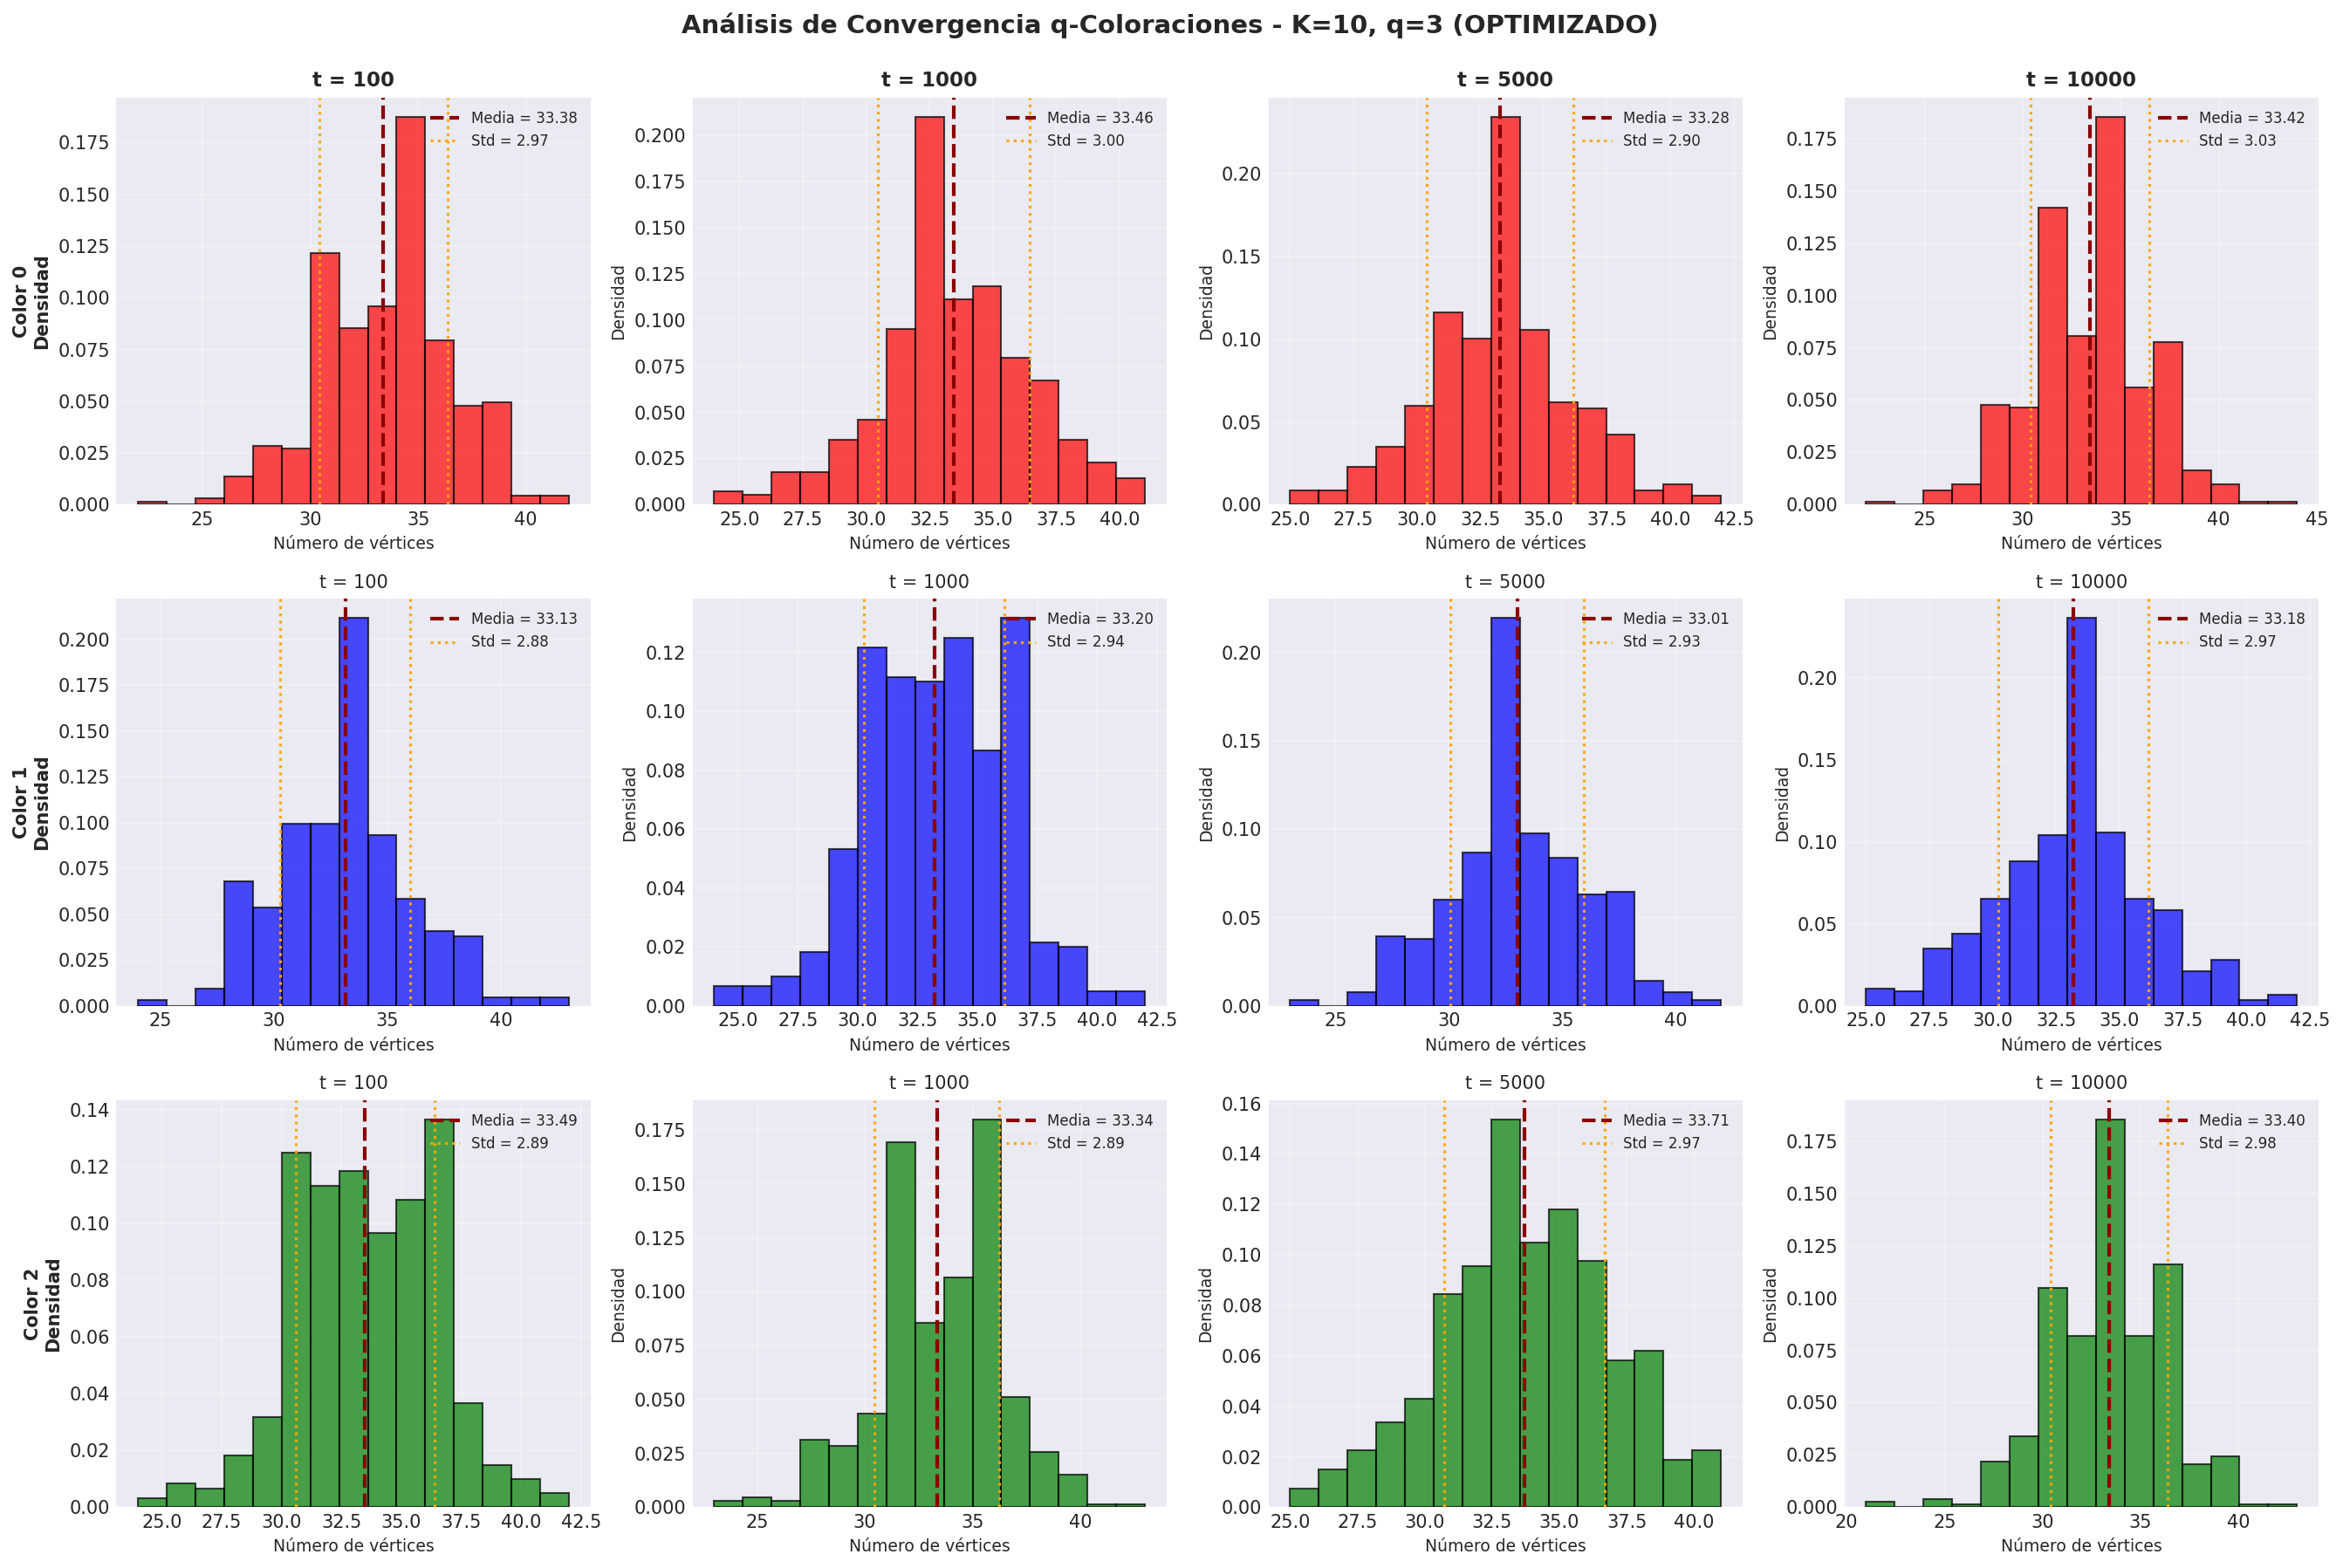
\includegraphics[width=0.85\textwidth]{../images/coloracion_convergencia_K10_q3.png}
\caption{Análisis de convergencia de q-coloraciones para $K=10$, $q=3$. Cada fila corresponde a un color, las columnas son tiempos $t \in \{100, 1000, 5000, 10000\}$. Las distribuciones convergen rápidamente y se mantienen estables.}
\end{figure}

\textbf{Estadísticas detalladas de convergencia:}

\begin{table}[H]
\centering
\begin{tabular}{|c|c|c|c|c|c|}
\hline
\textbf{Color} & \textbf{Tiempo} & \textbf{Media} & \textbf{Std} & \textbf{CV} & \textbf{Rango} \\
\hline
\multirow{4}{*}{Color 0} & $t=100$ & 33.38 & 2.97 & 0.089 & [22, 42] \\
& $t=1000$ & 33.46 & 3.00 & 0.090 & [24, 41] \\
& $t=5000$ & 33.28 & 2.90 & 0.087 & [25, 42] \\
& $t=10000$ & 33.42 & 3.03 & 0.091 & [22, 44] \\
\hline
\multirow{4}{*}{Color 1} & $t=100$ & 33.13 & 2.88 & 0.087 & [24, 43] \\
& $t=1000$ & 33.20 & 2.94 & 0.088 & [24, 42] \\
& $t=5000$ & 33.01 & 2.93 & 0.089 & [23, 42] \\
& $t=10000$ & 33.18 & 2.97 & 0.089 & [25, 42] \\
\hline
\multirow{4}{*}{Color 2} & $t=100$ & 33.49 & 2.89 & 0.086 & [24, 42] \\
& $t=1000$ & 33.34 & 2.89 & 0.087 & [23, 43] \\
& $t=5000$ & 33.71 & 2.97 & 0.088 & [25, 41] \\
& $t=10000$ & 33.40 & 2.98 & 0.089 & [21, 43] \\
\hline
\end{tabular}
\caption{Estadísticas de convergencia para q-coloraciones ($K=10$, $q=3$, 500 repeticiones).}
\end{table}

\textbf{Observaciones clave:} Las distribuciones convergen rápidamente (ya estables en $t \sim 1000$) con la media manteniéndose cerca de $K^2/q = 33.33$ vértices por color. La desviación estándar se estabiliza en $\sigma \approx 3$ para todos los tiempos, y el coeficiente de variación bajo ($CV \approx 0.089$) indica distribución uniforme. Los tres colores muestran comportamiento idéntico, evidenciando uniformidad perfecta.

\subsection{Análisis Comparativo}

\begin{figure}[H]
\centering
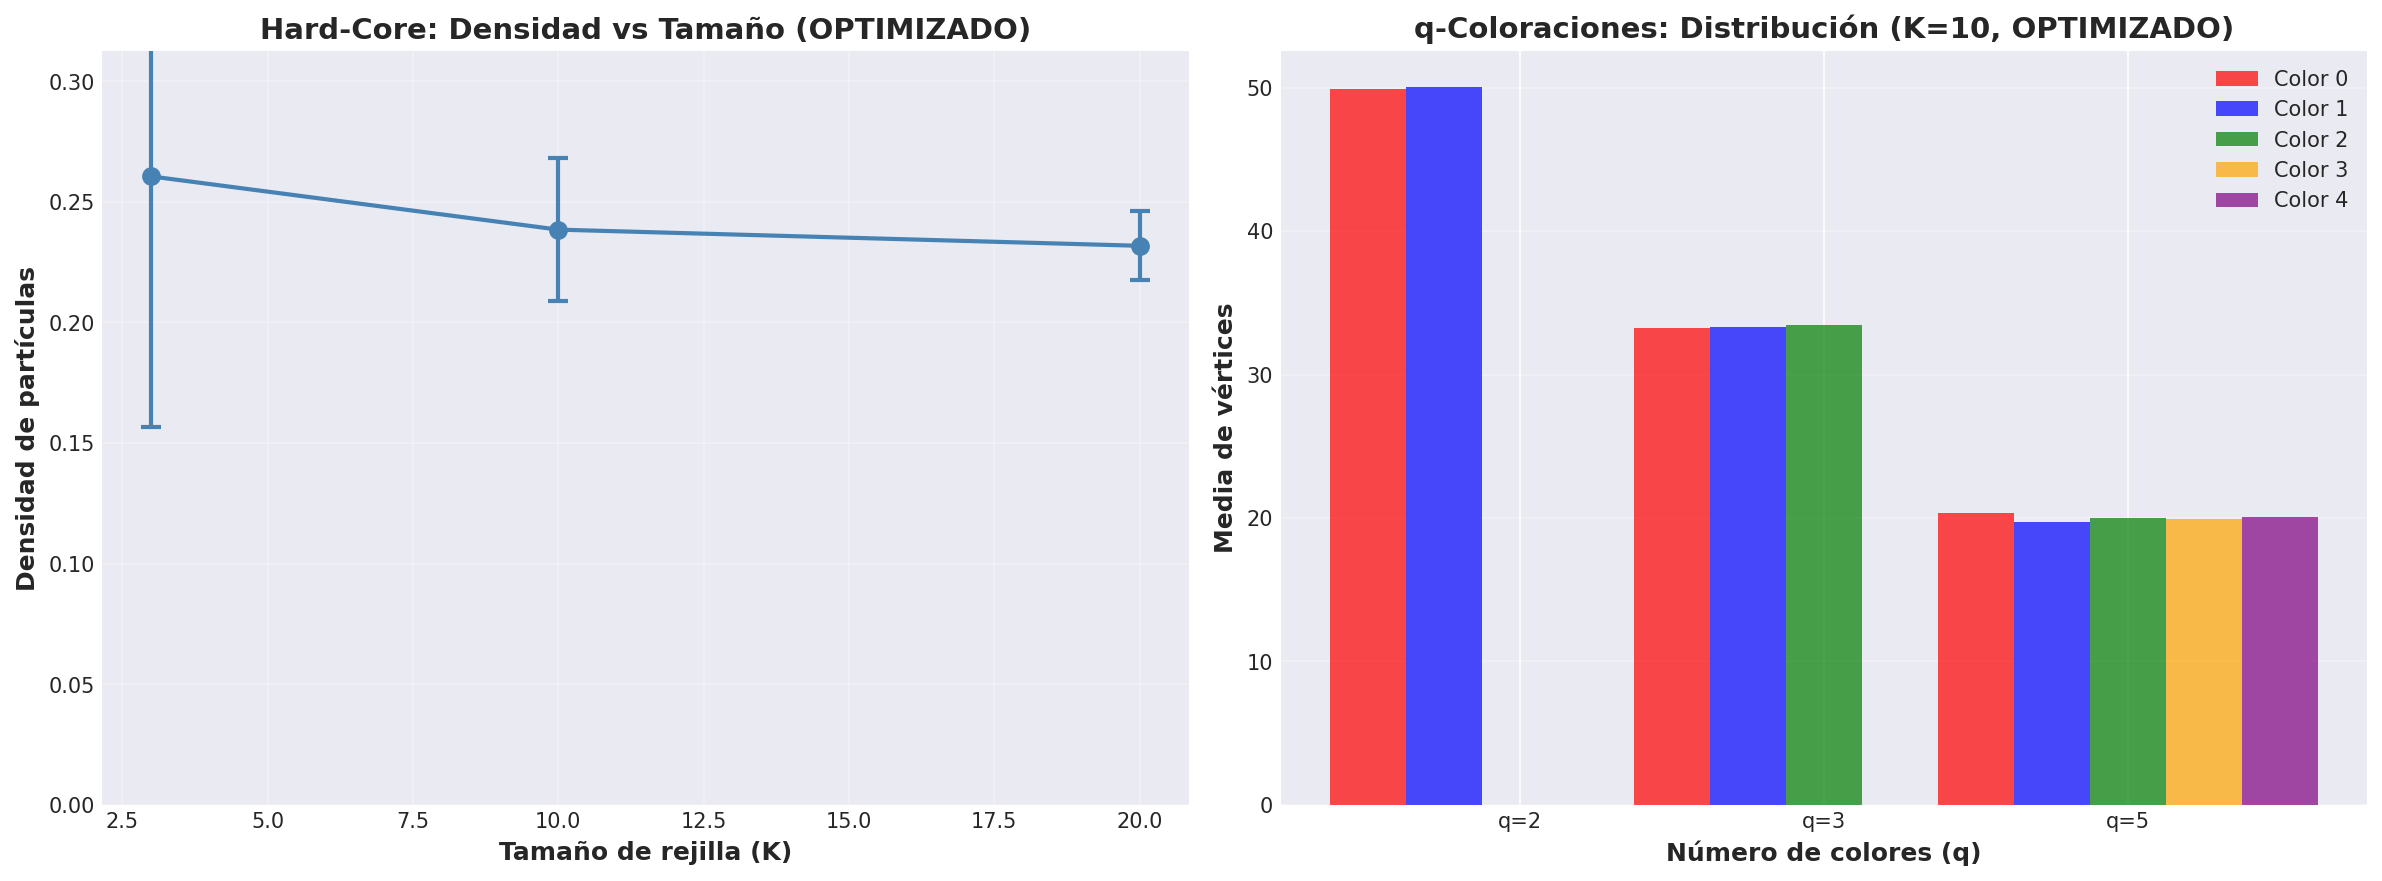
\includegraphics[width=0.9\textwidth]{../images/comparativo_general.png}
\caption{Análisis comparativo. Izquierda: Densidad Hard-Core vs tamaño de rejilla muestra convergencia a $\rho \approx 0.23$. Derecha: Distribución uniforme de colores para diferentes valores de $q$ en q-coloraciones.}
\end{figure}

\subsection{Resumen de Resultados}

Para el modelo Hard-Core se obtuvo una densidad promedio de $\rho \approx 0.24$ con convergencia en $\sim 1000$ iteraciones. Para q-coloraciones con $q=3$, la distribución de colores es aproximadamente uniforme con $\sim 33$ vértices por color. 
